\section{Test data generation for common cache}

\begin{figure}[h]
\centering
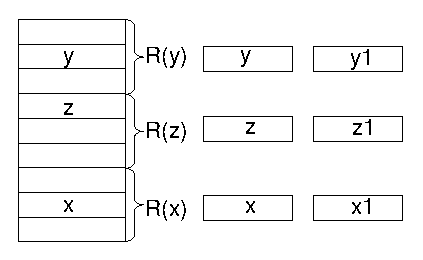
\includegraphics[width=2.5in]{common}
\caption{Common cache} \label{common_cache}
\end{figure}

This section consists of illustration only the constraints for
common cache.

Define function $R(x)$ as the same as for direct mapped cache.

Consider known test template for memory consisted of 3 regions
($R(x) = R(y) \leftrightarrow 3 | (x-y)$) of 2-associative cache:

LOAD x, y @ Hit

STORE u, z @ Miss

LOAD z, y @ Hit

Define unique variables (and $z'_0$ for evicted address):

LOAD $x_1, y_0$ @ Hit

STORE $u_0, z_0$ @ Miss $\rightarrow z'_0$

LOAD $z_1, y_0$ @ Hit

Define variables for initial cache state: $\alpha_1, \alpha_2$ for
the first region, $\beta_1, \beta_2$ for the second region,
$\gamma_1, \gamma_2$ for the third region. Constraints set is the
following:

$y_0 \in \{ \alpha_1, \alpha_2, \beta_1, \beta_2, \gamma_1, \gamma_2
\}$,

$z'_0 \in \{ \alpha_1, \alpha_2, \beta_1, \beta_2, \gamma_1,
\gamma_2 \}$,

$z_0 \notin \{ \alpha_1, \alpha_2, \beta_1, \beta_2, \gamma_1,
\gamma_2 \} \cap R(z'_0)$,

$y_0 \in \{ \alpha_1, \alpha_2, \beta_1, \beta_2, \gamma_1, \gamma_2
\} \cup \{z_0\} \setminus \{z'_0\}$,

$R(z_0) = R(z'_0)$,

$\alpha_1, \alpha_2, \beta_1, \beta_2, \gamma_1, \gamma_2$ --
different,

$R(\alpha_1) = R(\alpha_2)$,

$R(\beta_1) = R(\beta_2)$,

$R(\gamma_1) = R(\gamma_2)$,

$R(\alpha_1), R(\beta_1), R(\gamma_1)$ -- different

From disjunction for $lru(z'_0)$ (one clause is enough):

$z'_0 = \gamma_2 \wedge (\{ \alpha_1, \alpha_2, \beta_1, \beta_2,
\gamma_1, \gamma_2 \}\setminus \{z'_0\}) \cap R(z'_0) = \{y_0\} \cap
R(z'_0)$

$\vee$

...

Simplify:

$y_0 \in \{ \alpha_1, ..., \gamma_2 \}$,

$z'_0 \in \{ \alpha_1, ..., \gamma_2 \}$,

$z_0 \notin \{ \alpha_1, ..., \gamma_2 \} \cap R(z'_0)$,

$y_0 \in \{ \alpha_1, ..., \gamma_2, z_0 \} \setminus \{z'_0 \}$,

$R(z_0) = R(z'_0)$,

$z'_0 = \gamma_2$,

$\{ \gamma_1 \} = \{ y_0 \} \cap R(\gamma_2)$

$\alpha_1, \alpha_2, \beta_1, \beta_2, \gamma_1, \gamma_2$ --
different,

$R(\alpha_1) = R(\alpha_2)$,

$R(\beta_1) = R(\beta_2)$,

$R(\gamma_1) = R(\gamma_2)$,

$R(\alpha_1), R(\beta_1), R(\gamma_1)$ -- different

Further simplify:

$z'_0 = \gamma_2$,

$y_0 = \gamma_1$,

$z_0 \notin \{ \gamma_1, \gamma_2 \}$,

$R(z_0) = R(\gamma_2)$,

$\alpha_1, \alpha_2, \beta_1, \beta_2, \gamma_1, \gamma_2$ --
different,

$R(\alpha_1) = R(\alpha_2)$,

$R(\beta_1) = R(\beta_2)$,

$R(\gamma_1) = R(\gamma_2)$,

$R(\alpha_1), R(\beta_1), R(\gamma_1)$ -- different

Lets bit length of addresses is 8. So domain of all
variable-addresses is from 0 to 255. Satisfying constraints
variables can get the following values (these values are not
unique):

$\alpha_1 = 0, \alpha_2 = 3$,

$\beta_1 = 1, \beta_2 = 4$,

$\gamma_1 = 2, \gamma_2 = 5$,

$x_0 = 0, y_0 = 2, z_0 = 7, u_0 = 0$ .

Special algorithms can be used for solving constraints set. These
algorithms can take into account the following aspects:
\begin{itemize}
\item constraints can be solved symbolically;
\item all sets of addresses are finite and subset of all initial
cache state addresses union with evicting addresses.
\end{itemize}
